

\tikzset{every picture/.style={line width=0.75pt}} %set default line width to 0.75pt        

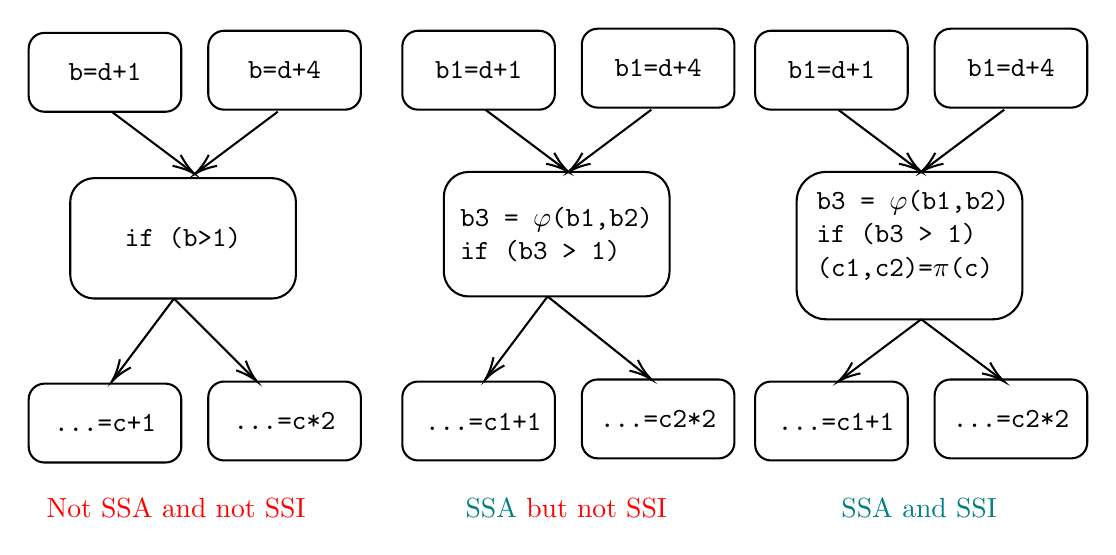
\begin{tikzpicture}[x=0.75pt,y=0.75pt,yscale=-1,xscale=1]
%uncomment if require: \path (0,314.6999969482422); %set diagram left start at 0, and has height of 314.6999969482422

%Rounded Rect [id:dp262243382651531] 
\draw   (10,188.6) .. controls (10,184.4) and (13.4,181) .. (17.6,181) -- (75.9,181) .. controls (80.1,181) and (83.5,184.4) .. (83.5,188.6) -- (83.5,211.4) .. controls (83.5,215.6) and (80.1,219) .. (75.9,219) -- (17.6,219) .. controls (13.4,219) and (10,215.6) .. (10,211.4) -- cycle ;
%Rounded Rect [id:dp4192314773958711] 
\draw   (96.5,187.6) .. controls (96.5,183.4) and (99.9,180) .. (104.1,180) -- (162.4,180) .. controls (166.6,180) and (170,183.4) .. (170,187.6) -- (170,210.4) .. controls (170,214.6) and (166.6,218) .. (162.4,218) -- (104.1,218) .. controls (99.9,218) and (96.5,214.6) .. (96.5,210.4) -- cycle ;
%Rounded Rect [id:dp14874696406611254] 
\draw   (30,93.6) .. controls (30,87.19) and (35.19,82) .. (41.6,82) -- (127.15,82) .. controls (133.56,82) and (138.75,87.19) .. (138.75,93.6) -- (138.75,128.4) .. controls (138.75,134.81) and (133.56,140) .. (127.15,140) -- (41.6,140) .. controls (35.19,140) and (30,134.81) .. (30,128.4) -- cycle ;
%Straight Lines [id:da8036054523449865] 
\draw    (80,140) -- (51.2,178.4) ;
\draw [shift={(50,180)}, rotate = 306.87] [color={rgb, 255:red, 0; green, 0; blue, 0 }  ][line width=0.75]    (10.93,-3.29) .. controls (6.95,-1.4) and (3.31,-0.3) .. (0,0) .. controls (3.31,0.3) and (6.95,1.4) .. (10.93,3.29)   ;

%Straight Lines [id:da9462543361304327] 
\draw    (80,140) -- (118.59,178.59) ;
\draw [shift={(120,180)}, rotate = 225] [color={rgb, 255:red, 0; green, 0; blue, 0 }  ][line width=0.75]    (10.93,-3.29) .. controls (6.95,-1.4) and (3.31,-0.3) .. (0,0) .. controls (3.31,0.3) and (6.95,1.4) .. (10.93,3.29)   ;

%Rounded Rect [id:dp804370127764321] 
\draw   (190,187.6) .. controls (190,183.4) and (193.4,180) .. (197.6,180) -- (255.9,180) .. controls (260.1,180) and (263.5,183.4) .. (263.5,187.6) -- (263.5,210.4) .. controls (263.5,214.6) and (260.1,218) .. (255.9,218) -- (197.6,218) .. controls (193.4,218) and (190,214.6) .. (190,210.4) -- cycle ;
%Rounded Rect [id:dp054537017000311994] 
\draw   (276.5,186.6) .. controls (276.5,182.4) and (279.9,179) .. (284.1,179) -- (342.4,179) .. controls (346.6,179) and (350,182.4) .. (350,186.6) -- (350,209.4) .. controls (350,213.6) and (346.6,217) .. (342.4,217) -- (284.1,217) .. controls (279.9,217) and (276.5,213.6) .. (276.5,209.4) -- cycle ;
%Rounded Rect [id:dp9347541053691467] 
\draw   (210,91) .. controls (210,84.37) and (215.37,79) .. (222,79) -- (306.75,79) .. controls (313.38,79) and (318.75,84.37) .. (318.75,91) -- (318.75,127) .. controls (318.75,133.63) and (313.38,139) .. (306.75,139) -- (222,139) .. controls (215.37,139) and (210,133.63) .. (210,127) -- cycle ;
%Straight Lines [id:da09161146890023963] 
\draw    (260,139) -- (231.2,177.4) ;
\draw [shift={(230,179)}, rotate = 306.87] [color={rgb, 255:red, 0; green, 0; blue, 0 }  ][line width=0.75]    (10.93,-3.29) .. controls (6.95,-1.4) and (3.31,-0.3) .. (0,0) .. controls (3.31,0.3) and (6.95,1.4) .. (10.93,3.29)   ;

%Straight Lines [id:da9445970974561072] 
\draw    (260,139) -- (308.44,177.75) ;
\draw [shift={(310,179)}, rotate = 218.66] [color={rgb, 255:red, 0; green, 0; blue, 0 }  ][line width=0.75]    (10.93,-3.29) .. controls (6.95,-1.4) and (3.31,-0.3) .. (0,0) .. controls (3.31,0.3) and (6.95,1.4) .. (10.93,3.29)   ;

%Rounded Rect [id:dp4977532430387589] 
\draw   (10,19.6) .. controls (10,15.4) and (13.4,12) .. (17.6,12) -- (75.9,12) .. controls (80.1,12) and (83.5,15.4) .. (83.5,19.6) -- (83.5,42.4) .. controls (83.5,46.6) and (80.1,50) .. (75.9,50) -- (17.6,50) .. controls (13.4,50) and (10,46.6) .. (10,42.4) -- cycle ;
%Rounded Rect [id:dp5889626886983321] 
\draw   (96.5,18.6) .. controls (96.5,14.4) and (99.9,11) .. (104.1,11) -- (162.4,11) .. controls (166.6,11) and (170,14.4) .. (170,18.6) -- (170,41.4) .. controls (170,45.6) and (166.6,49) .. (162.4,49) -- (104.1,49) .. controls (99.9,49) and (96.5,45.6) .. (96.5,41.4) -- cycle ;
%Straight Lines [id:da038881567998766964] 
\draw    (50,50) -- (88.4,78.8) ;
\draw [shift={(90,80)}, rotate = 216.87] [color={rgb, 255:red, 0; green, 0; blue, 0 }  ][line width=0.75]    (10.93,-3.29) .. controls (6.95,-1.4) and (3.31,-0.3) .. (0,0) .. controls (3.31,0.3) and (6.95,1.4) .. (10.93,3.29)   ;

%Straight Lines [id:da9119956977469609] 
\draw    (130,50) -- (91.6,78.8) ;
\draw [shift={(90,80)}, rotate = 323.13] [color={rgb, 255:red, 0; green, 0; blue, 0 }  ][line width=0.75]    (10.93,-3.29) .. controls (6.95,-1.4) and (3.31,-0.3) .. (0,0) .. controls (3.31,0.3) and (6.95,1.4) .. (10.93,3.29)   ;

%Rounded Rect [id:dp450867564409416] 
\draw   (190,18.6) .. controls (190,14.4) and (193.4,11) .. (197.6,11) -- (255.9,11) .. controls (260.1,11) and (263.5,14.4) .. (263.5,18.6) -- (263.5,41.4) .. controls (263.5,45.6) and (260.1,49) .. (255.9,49) -- (197.6,49) .. controls (193.4,49) and (190,45.6) .. (190,41.4) -- cycle ;
%Rounded Rect [id:dp06195868427554574] 
\draw   (276.5,17.6) .. controls (276.5,13.4) and (279.9,10) .. (284.1,10) -- (342.4,10) .. controls (346.6,10) and (350,13.4) .. (350,17.6) -- (350,40.4) .. controls (350,44.6) and (346.6,48) .. (342.4,48) -- (284.1,48) .. controls (279.9,48) and (276.5,44.6) .. (276.5,40.4) -- cycle ;
%Straight Lines [id:da334726632196392] 
\draw    (230,49) -- (268.4,77.8) ;
\draw [shift={(270,79)}, rotate = 216.87] [color={rgb, 255:red, 0; green, 0; blue, 0 }  ][line width=0.75]    (10.93,-3.29) .. controls (6.95,-1.4) and (3.31,-0.3) .. (0,0) .. controls (3.31,0.3) and (6.95,1.4) .. (10.93,3.29)   ;

%Straight Lines [id:da41014358467548495] 
\draw    (310,49) -- (271.6,77.8) ;
\draw [shift={(270,79)}, rotate = 323.13] [color={rgb, 255:red, 0; green, 0; blue, 0 }  ][line width=0.75]    (10.93,-3.29) .. controls (6.95,-1.4) and (3.31,-0.3) .. (0,0) .. controls (3.31,0.3) and (6.95,1.4) .. (10.93,3.29)   ;

%Rounded Rect [id:dp3691248800233007] 
\draw   (360,187.6) .. controls (360,183.4) and (363.4,180) .. (367.6,180) -- (425.9,180) .. controls (430.1,180) and (433.5,183.4) .. (433.5,187.6) -- (433.5,210.4) .. controls (433.5,214.6) and (430.1,218) .. (425.9,218) -- (367.6,218) .. controls (363.4,218) and (360,214.6) .. (360,210.4) -- cycle ;
%Rounded Rect [id:dp19131836124451396] 
\draw   (446.5,186.6) .. controls (446.5,182.4) and (449.9,179) .. (454.1,179) -- (512.4,179) .. controls (516.6,179) and (520,182.4) .. (520,186.6) -- (520,209.4) .. controls (520,213.6) and (516.6,217) .. (512.4,217) -- (454.1,217) .. controls (449.9,217) and (446.5,213.6) .. (446.5,209.4) -- cycle ;
%Rounded Rect [id:dp14926613816841217] 
\draw   (380,93.2) .. controls (380,85.36) and (386.36,79) .. (394.2,79) -- (474.55,79) .. controls (482.39,79) and (488.75,85.36) .. (488.75,93.2) -- (488.75,135.8) .. controls (488.75,143.64) and (482.39,150) .. (474.55,150) -- (394.2,150) .. controls (386.36,150) and (380,143.64) .. (380,135.8) -- cycle ;
%Straight Lines [id:da6856746540157947] 
\draw    (440,150) -- (401.6,178.8) ;
\draw [shift={(400,180)}, rotate = 323.13] [color={rgb, 255:red, 0; green, 0; blue, 0 }  ][line width=0.75]    (10.93,-3.29) .. controls (6.95,-1.4) and (3.31,-0.3) .. (0,0) .. controls (3.31,0.3) and (6.95,1.4) .. (10.93,3.29)   ;

%Straight Lines [id:da6670526861113566] 
\draw    (440,150) -- (478.4,178.8) ;
\draw [shift={(480,180)}, rotate = 216.87] [color={rgb, 255:red, 0; green, 0; blue, 0 }  ][line width=0.75]    (10.93,-3.29) .. controls (6.95,-1.4) and (3.31,-0.3) .. (0,0) .. controls (3.31,0.3) and (6.95,1.4) .. (10.93,3.29)   ;

%Rounded Rect [id:dp00671566926016387] 
\draw   (360,18.6) .. controls (360,14.4) and (363.4,11) .. (367.6,11) -- (425.9,11) .. controls (430.1,11) and (433.5,14.4) .. (433.5,18.6) -- (433.5,41.4) .. controls (433.5,45.6) and (430.1,49) .. (425.9,49) -- (367.6,49) .. controls (363.4,49) and (360,45.6) .. (360,41.4) -- cycle ;
%Rounded Rect [id:dp8281541882214426] 
\draw   (446.5,17.6) .. controls (446.5,13.4) and (449.9,10) .. (454.1,10) -- (512.4,10) .. controls (516.6,10) and (520,13.4) .. (520,17.6) -- (520,40.4) .. controls (520,44.6) and (516.6,48) .. (512.4,48) -- (454.1,48) .. controls (449.9,48) and (446.5,44.6) .. (446.5,40.4) -- cycle ;
%Straight Lines [id:da8015873618397712] 
\draw    (400,49) -- (438.4,77.8) ;
\draw [shift={(440,79)}, rotate = 216.87] [color={rgb, 255:red, 0; green, 0; blue, 0 }  ][line width=0.75]    (10.93,-3.29) .. controls (6.95,-1.4) and (3.31,-0.3) .. (0,0) .. controls (3.31,0.3) and (6.95,1.4) .. (10.93,3.29)   ;

%Straight Lines [id:da2656759697778148] 
\draw    (480,49) -- (441.6,77.8) ;
\draw [shift={(440,79)}, rotate = 323.13] [color={rgb, 255:red, 0; green, 0; blue, 0 }  ][line width=0.75]    (10.93,-3.29) .. controls (6.95,-1.4) and (3.31,-0.3) .. (0,0) .. controls (3.31,0.3) and (6.95,1.4) .. (10.93,3.29)   ;


% Text Node
\draw (46.75,200) node  [align=left] {{\tt ...=c+1}};
% Text Node
\draw (133.25,199) node  [align=left] {{\tt ...=c*2}};
% Text Node
\draw (84.38,111) node  [align=left] {{\tt if (b>1)}};
% Text Node
\draw (264.38,109) node  [align=left] {{\tt b3 = }$\displaystyle \varphi ${\tt (b1,b2)}\\{\tt if (b3 > 1)}};
% Text Node
\draw (229,199.5) node  [align=left] {{\tt ...=c1+1}};
% Text Node
\draw (313.25,198) node  [align=left] {{\tt ...=c2*2}};
% Text Node
\draw (46.75,31) node  [align=left] {{\tt b=d+1}};
% Text Node
\draw (133.25,30) node  [align=left] {{\tt b=d+4}};
% Text Node
\draw (226.75,30) node  [align=left] {{\tt b1=d+1}};
% Text Node
\draw (313.25,29) node  [align=left] {{\tt b1=d+4}};
% Text Node
\draw (81,241) node  [align=left] {\textcolor{red}{Not SSA and not SSI}};
% Text Node
\draw (269,241) node  [align=left] {\textcolor{teal}{SSA} \textcolor{red}{but not SSI}};
% Text Node
\draw (436,109.5) node  [align=left] {{\tt b3 = }$\displaystyle \varphi ${\tt (b1,b2)}\\{\tt if (b3 > 1)}\\{\tt (c1,c2)=}$\displaystyle \pi ${\tt (c)}};
% Text Node
\draw (399,199.5) node  [align=left] {{\tt ...=c1+1}};
% Text Node
\draw (483.25,198) node  [align=left] {{\tt ...=c2*2}};
% Text Node
\draw (396.75,30) node  [align=left] {{\tt b1=d+1}};
% Text Node
\draw (483.25,29) node  [align=left] {{\tt b1=d+4}};
% Text Node
\draw (439,241) node  [align=left] {\textcolor{teal}{SSA and SSI}};


\end{tikzpicture}
